\chapter{Description of research projects}
\label{chap:rationale}

Locomotion is thought to be a tightly controlled behaviour, ensuring good sensory performance, especially visual, and reducing energy expenditure \autocites{Benichou2011IntermittentStrategies, Kramer2001}. Whether this is the case in the wood ant \textit{Formica rufa} remains unknown, despite many aspects of ant locomotion having been well studied \autocites{Lipp2005, Wahl2015}. The wood ant is an eusocial insect capable of using vision for navigation \autocite{Harris2007} and associative learning \autocite{Fernandes2017a}. Furthermore, other ant species have been found able to use optic flow for path integration (\textit{Cataglyphis}, \citealt{Ronacher1995, Pfeffer2016}). It could thus be speculated that vision actively controls general walking features such as speed, duration and pausing in the wood ant, \textit{Formica rufa} (like bees control speed, \cite{Schone1996, Linander2015}). We ask the following question: Does control of walking speed and pausing depend on the presence and speed of optic flow?

A promising approach for performing behavioural experiments in a laboratory setting is the use of virtual reality. Insects have recently been shown to exhibit naturalistic behaviour in closed-loop within a virtual environment \autocites{Takalo2012, Buatois2017, Seelig2010}. Such setups allow data sampling at precise temporal and spatial resolution whilst animals walk unrestricted for long periods of time. They further enable the recording of brain activity directly, either by electrophysiological recordings or calcium imaging \autocite{Seelig2010}. However, despite continued efforts from multiple laboratories it has not yet been possible to make a setup in which ants will readily behave within closed-loop. Nevertheless, we set out to develop a virtual reality paradigm for wood ants (\textit{Formica rufa}). We propose a paradigm based on a modified closed-loop version of the trackball setup by \citeauthor{Dahmen2017} (\citeyear{Dahmen2017}) combined with the virtual reality software developed by \citeauthor{Aronov2014b} (\citeyear{Aronov2014b}).

\begin{figure}[h]
    \centering
    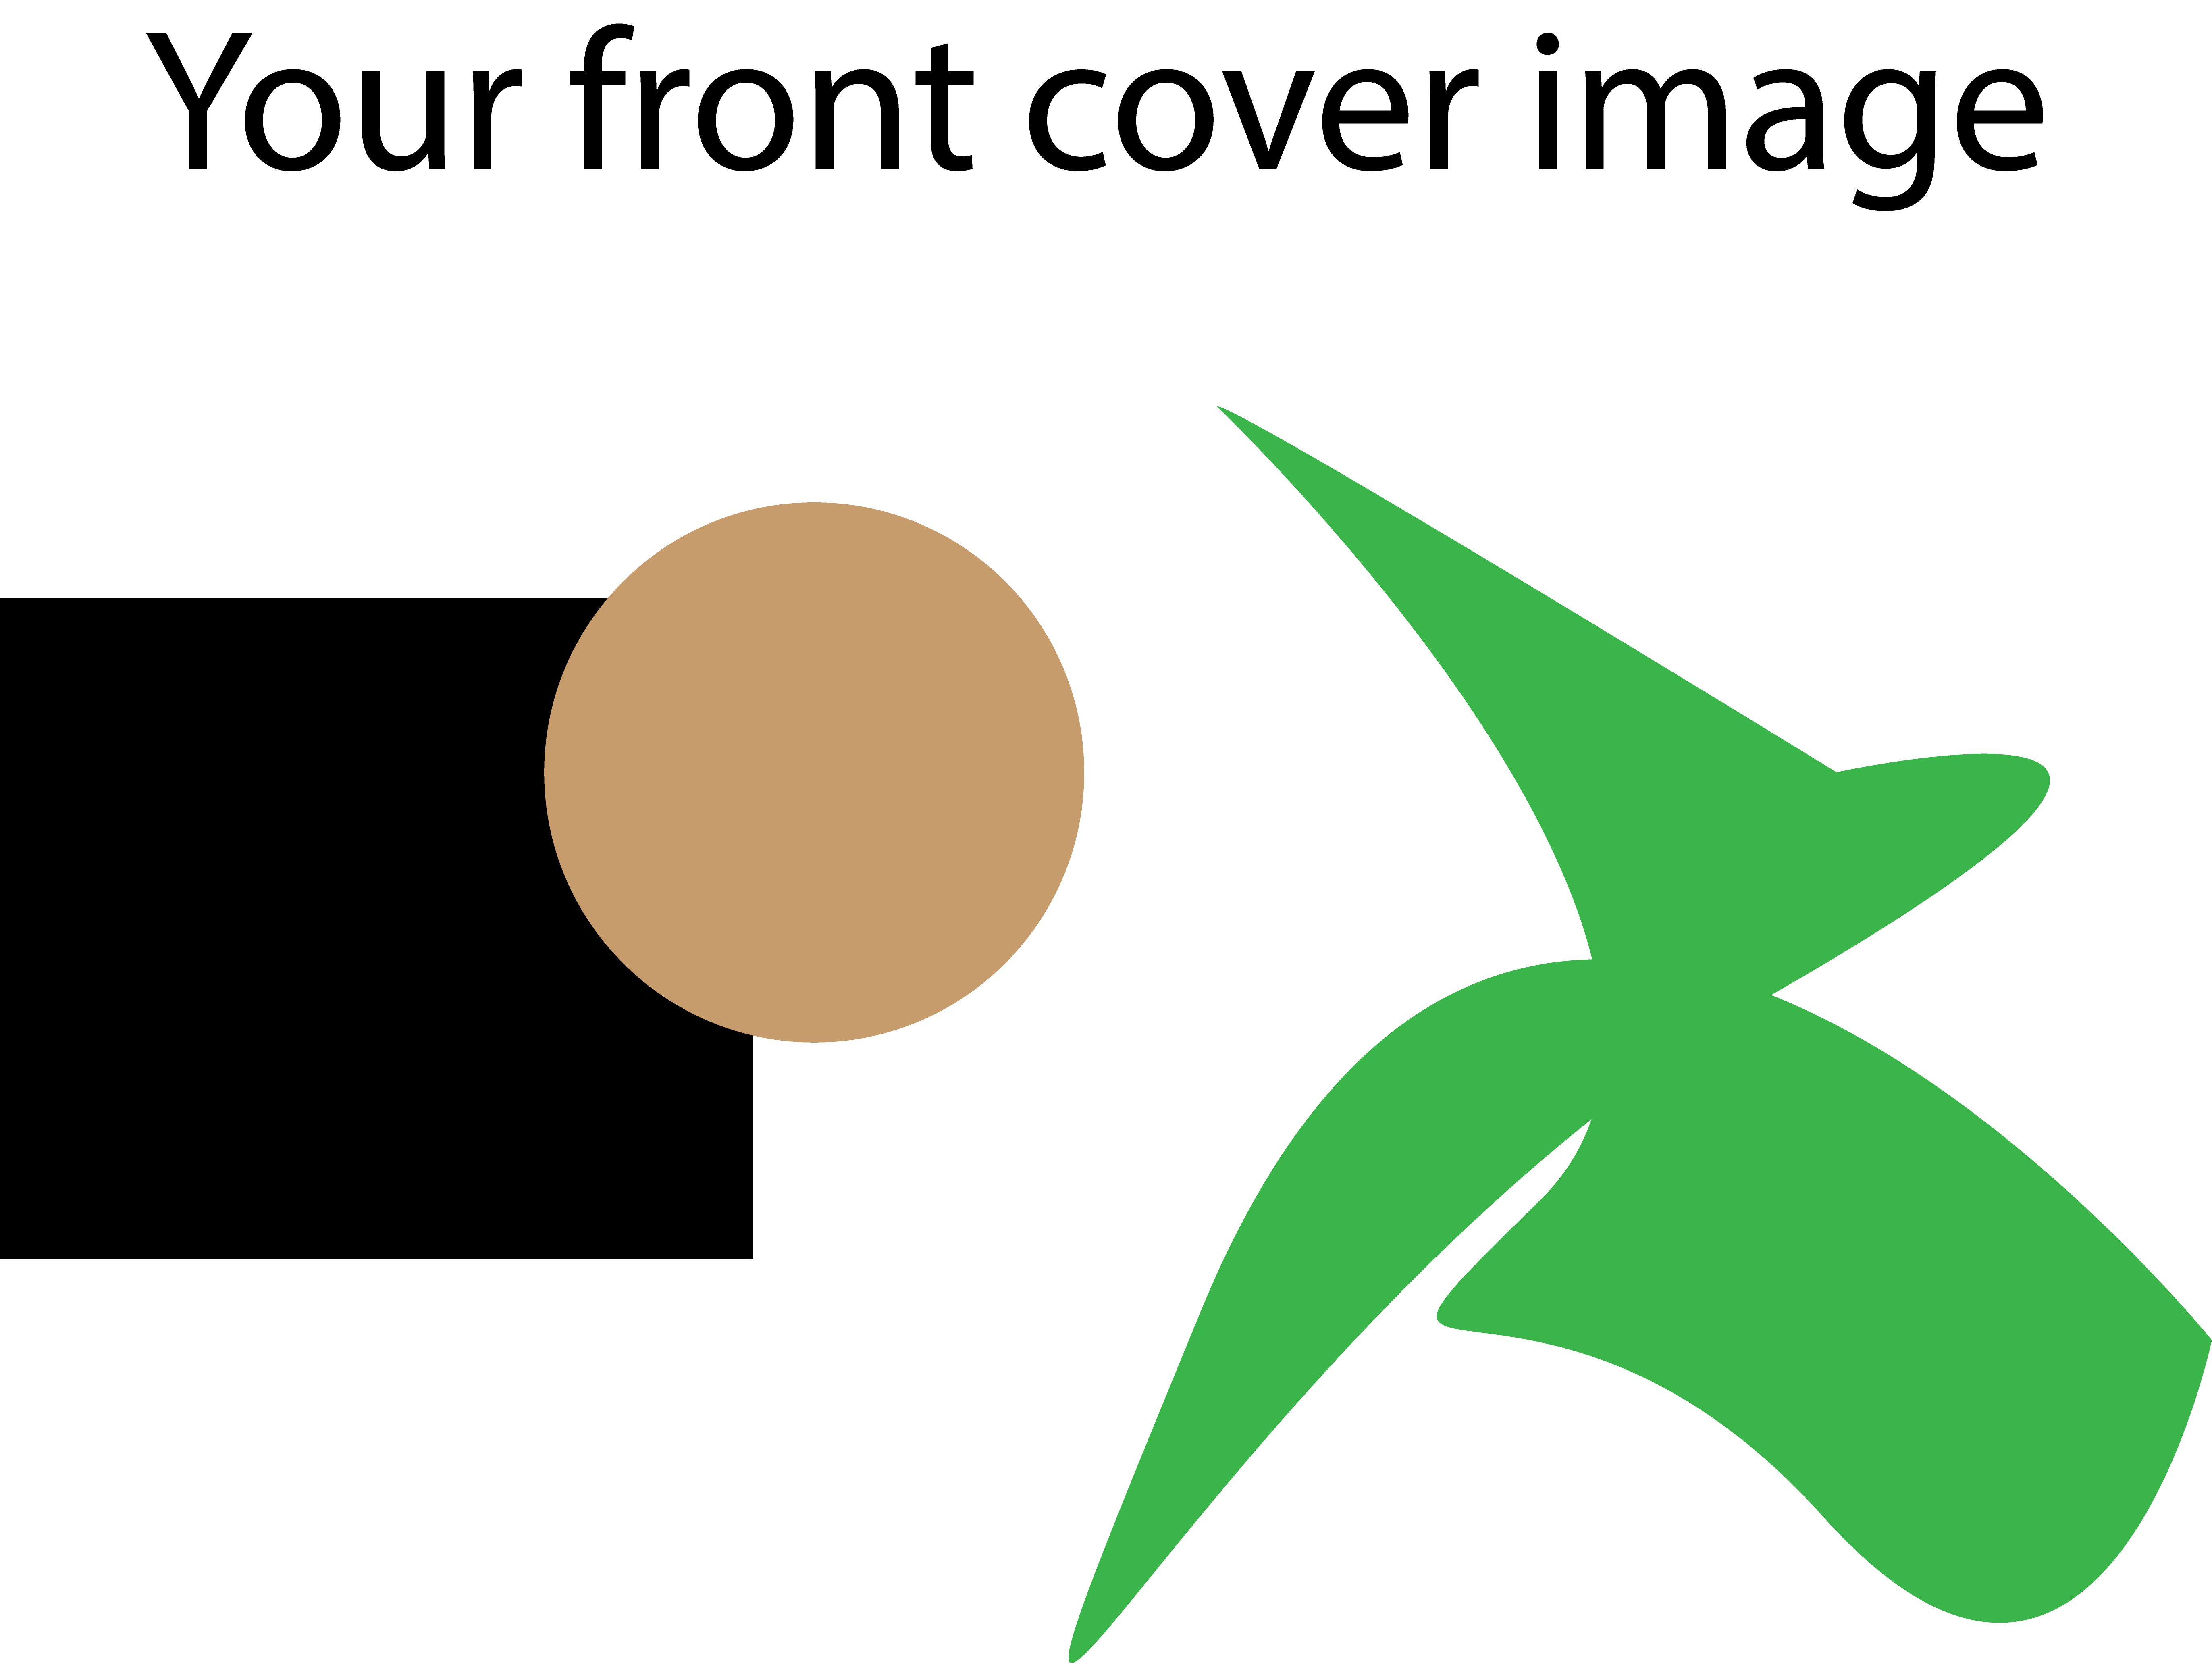
\includegraphics[width=100mm]{theme/cover_image.png}
    \caption{Image example}
    \label{fig:image_example}
\end{figure}